% Standalone source for Figure: Mininet emulation backend (E4).
% Compile with: pdflatex mininet_architecture.tex  (produces mininet_architecture.pdf)
\documentclass[tikz,border=4pt]{standalone}
\usepackage{amsmath,amssymb}
\usetikzlibrary{positioning,arrows.meta,fit,backgrounds,calc}
\definecolor{blue1}{HTML}{2A78D6}
\definecolor{orange1}{HTML}{EB6834}
\definecolor{aqua1}{HTML}{1BAF7A}
\definecolor{ink2}{HTML}{52514E}
\begin{document}
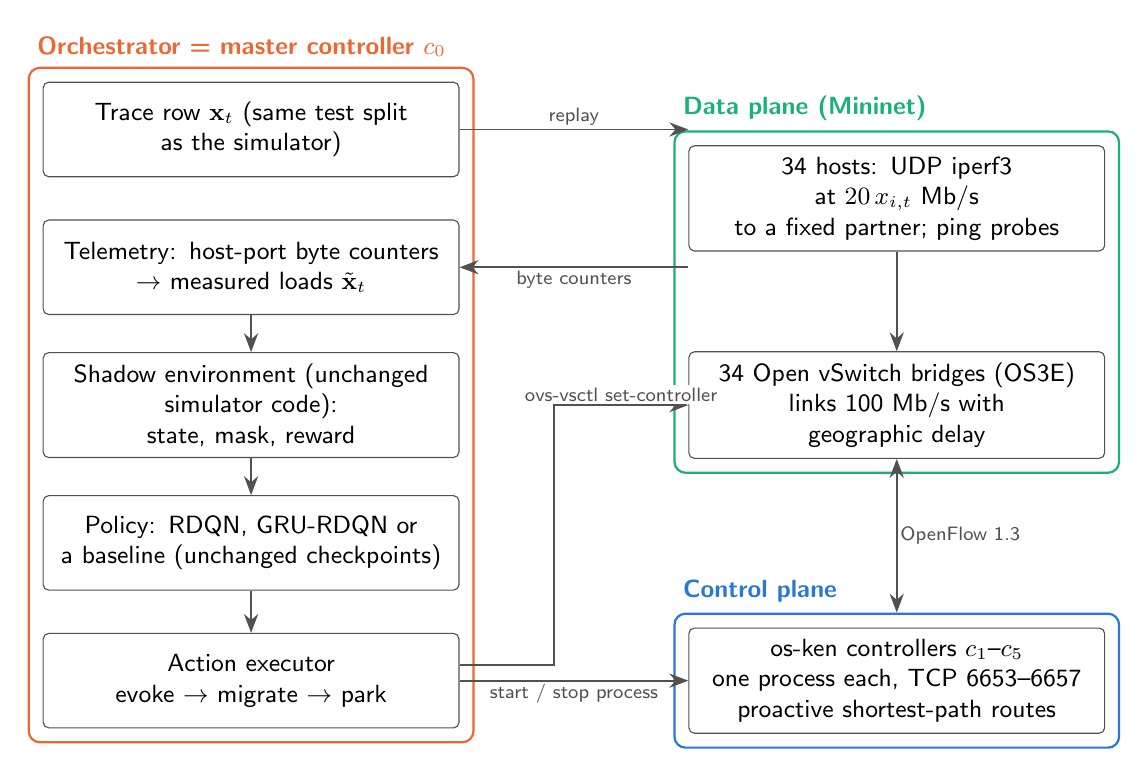
\begin{tikzpicture}[
  font=\sffamily\small,
  every node/.append style={execute at begin node={\hyphenpenalty 10000\relax}},
  box/.style={draw=ink2, rounded corners=2pt, align=center, fill=white,
              minimum height=12mm, inner sep=4pt, text width=#1},
  box/.default=50mm,
  grp/.style={draw=#1, rounded corners=4pt, line width=0.8pt, inner sep=5pt},
  lbl/.style={font=\sffamily\bfseries\small, anchor=south west},
  arr/.style={-{Stealth[length=2.4mm]}, line width=0.7pt, draw=ink2},
  note/.style={font=\sffamily\scriptsize, text=ink2, align=center, fill=white, inner sep=1pt},
]
% ---------------- left column: orchestrator (master controller c0)
\node[box] (trace)  at (0, 0)     {Trace row $\mathbf{x}_t$ (same test split\\as the simulator)};
\node[box] (tel)    at (0,-1.75)  {Telemetry: host-port byte counters\\$\rightarrow$ measured loads $\tilde{\mathbf{x}}_t$};
\node[box] (shadow) at (0,-3.5)   {Shadow environment (unchanged\\simulator code): state, mask, reward};
\node[box] (policy) at (0,-5.25)  {Policy: RDQN, \mbox{GRU-RDQN} or\\a baseline (unchanged checkpoints)};
\node[box] (exec)   at (0,-7.0)   {Action executor\\evoke $\rightarrow$ migrate $\rightarrow$ park};
\draw[arr] (tel) -- (shadow);
\draw[arr] (shadow) -- (policy);
\draw[arr] (policy) -- (exec);
\begin{scope}[on background layer]
  \node[grp=orange1, fit=(trace)(tel)(shadow)(policy)(exec)] (orch) {};
\end{scope}
\node[lbl, text=orange1] at (orch.north west) {Orchestrator = master controller $c_0$};

% ---------------- right column: data plane and control plane
\node[box] (hosts) at (8.2, -0.875) {34 hosts: UDP iperf3 at $20\,x_{i,t}$ Mb/s\\to a fixed partner; ping probes};
\node[box] (ovs)   at (8.2, -3.5)   {34 Open vSwitch bridges (OS3E)\\links 100 Mb/s with geographic delay};
\begin{scope}[on background layer]
  \node[grp=aqua1, fit=(hosts)(ovs)] (dp) {};
\end{scope}
\node[lbl, text=aqua1] at (dp.north west) {Data plane (Mininet)};

\node[box] (ctl) at (8.2, -7.0) {os-ken controllers $c_1$--$c_5$\\one process each, \mbox{TCP 6653--6657}\\proactive shortest-path routes};
\begin{scope}[on background layer]
  \node[grp=blue1, fit=(ctl)] (cp) {};
\end{scope}
\node[lbl, text=blue1] at (cp.north west) {Control plane};

% ---------------- arrows
\draw[arr] (trace.east) -- node[note, above] {replay} (trace.east -| hosts.west);
\draw[arr] (hosts.west |- tel.east) -- node[note, below] {byte counters} (tel.east);
\draw[arr] (hosts) -- (ovs);
\draw[arr] (exec.east) -- node[note, below] {start / stop process} (ctl.west);
\draw[arr] ([yshift=2mm]exec.east) -- ++(12mm,0) |- node[note, pos=0.75, above] {ovs-vsctl set-controller} (ovs.west);
\draw[arr, {Stealth[length=2.4mm]}-{Stealth[length=2.4mm]}] (ovs.south) -- node[note, right] {OpenFlow 1.3} (cp.north -| ovs.south);
\end{tikzpicture}
\end{document}
